% !TEX program = xelatex
\documentclass[10pt,a4paper,twocolumn,fontset=fandol]{ctexart}

\usepackage[a4paper,margin=2.0cm]{geometry}
\usepackage{graphicx}
\usepackage{booktabs}
\usepackage{amsmath,amssymb}
\usepackage{multirow}
\usepackage{array}
\usepackage{tabularx}
\usepackage{float}
\usepackage{caption}
\usepackage{subcaption}
\usepackage{xcolor}
\usepackage{enumitem}
\usepackage{hyperref}
\usepackage{tikz}
\usetikzlibrary{arrows.meta,positioning,shapes.geometric,fit,backgrounds,calc}

\definecolor{paperbg}{HTML}{F7F5F2}
\definecolor{ink}{HTML}{222222}
\definecolor{bluegray}{HTML}{A8B4C8}
\definecolor{steel}{HTML}{6C8EAD}
\definecolor{sand}{HTML}{D6A46A}
\definecolor{clay}{HTML}{D96C4F}
\definecolor{mist}{HTML}{EEF1F5}
\definecolor{linegray}{HTML}{D9DDE3}

\hypersetup{
  colorlinks=true,
  linkcolor=blue!40!black,
  citecolor=blue!40!black,
  urlcolor=blue!50!black
}

\captionsetup{font=small,labelfont=bf}
\setlength{\columnsep}{0.72cm}
\setlength{\parindent}{2em}
\setlength{\parskip}{0pt}
\linespread{1.12}
\raggedbottom
\pagestyle{plain}
\newcolumntype{Y}{>{\raggedright\arraybackslash}X}

\tikzset{
  paper diagram/.style={
    font=\small,
    >={Latex[length=2.1mm]},
    line cap=round,
    line join=round
  },
  stagebox/.style={
    draw=ink!90,
    rounded corners=4pt,
    line width=0.8pt,
    align=center,
    fill=paperbg,
    inner sep=5.5pt
  },
  bluebox/.style={stagebox, fill=bluegray!28},
  tealbox/.style={stagebox, fill=steel!22},
  warmbox/.style={stagebox, fill=sand!30},
  accentbox/.style={stagebox, fill=clay!22},
  tracebox/.style={stagebox, fill=mist, draw=ink!75},
  panelbox/.style={
    draw=ink!18,
    rounded corners=7pt,
    line width=0.55pt,
    fill=mist!52,
    inner xsep=8pt,
    inner ysep=8pt
  },
  paneltitle/.style={
    font=\bfseries\footnotesize,
    text=ink!72,
    inner sep=1pt
  },
  badge/.style={
    circle,
    draw=ink!70,
    fill=ink!82,
    text=white,
    font=\scriptsize\bfseries,
    inner sep=1.4pt,
    minimum size=4.2mm
  },
  mini tag/.style={
    rounded corners=2pt,
    draw=ink!30,
    fill=paperbg,
    font=\scriptsize,
    text=ink!80,
    inner xsep=3.2pt,
    inner ysep=1.6pt
  },
  flowcard/.style={
    stagebox,
    rounded corners=7pt,
    minimum height=1.04cm,
    text width=2.15cm,
    inner sep=6pt
  },
  iconnode/.style={
    circle,
    draw=white,
    line width=0.7pt,
    fill=ink!78,
    text=white,
    font=\scriptsize\bfseries,
    minimum size=5.2mm,
    inner sep=0pt
  },
  rolebubble/.style={
    circle,
    draw=ink!72,
    line width=0.8pt,
    align=center,
    font=\footnotesize,
    text width=1.05cm,
    minimum size=1.28cm,
    inner sep=1pt
  },
  auditdot/.style={
    circle,
    draw=ink!60,
    fill=paperbg,
    minimum size=2.4mm,
    inner sep=0pt
  },
  decisionbox/.style={
    draw=ink!90,
    diamond,
    aspect=2,
    line width=0.8pt,
    align=center,
    fill=clay!16,
    inner sep=1.8pt
  },
  flowarrow/.style={->, draw=ink!88, line width=0.85pt},
  mainarrow/.style={-{Latex[length=2.8mm,width=1.8mm]}, draw=ink!86, line width=1.05pt},
  softarrow/.style={-{Latex[length=2.2mm,width=1.3mm]}, draw=ink!56, line width=0.7pt},
  tracearrow/.style={->, draw=ink!58, dashed, line width=0.75pt},
  auditline/.style={draw=ink!45, dashed, line width=0.65pt}
}

\newcommand{\TitleCN}{面向受限能力命名空间的单智能体与多智能体协同语义路由方法}
\newcommand{\TitleEN}{A Single-Agent and Multi-Agent Collaborative Semantic Routing Method for Constrained Capability Namespaces}

\begin{document}

\twocolumn[
\begin{@twocolumnfalse}
\begin{center}
{\zihao{3}\bfseries \TitleCN\par}
\vspace{0.8em}
{\zihao{-4} 作者信息待补\par}
\vspace{0.3em}
{\small 单位信息待补\par}
\vspace{0.5em}
{\small 第一作者信息和通讯作者信息待补。}
\end{center}

\vspace{0.6em}
\noindent\textbf{摘\ \ 要}\quad
在受限能力命名空间下的智能体服务调用过程中，自然语言请求需要被准确映射到对应能力地址，否则容易造成主能力错选、相关能力遗漏和后续调用失败。本文聚焦服务调用链路中的能力地址语义路由问题，并将下游执行接口作为系统衔接模块保留。针对现有规则路由在跨域重叠、层级冲突和多意图请求上区分能力不足，以及一步式大模型方法在固定候选集合内部缺少稳定比较依据的问题，提出一种单智能体与多智能体协同语义路由方法。该方法首先在统一能力命名空间内构造候选集合，然后由单智能体结构化语义路由完成主能力选择与相关能力识别；针对低置信、高风险和多意图冲突样本，触发多智能体职责化协作复核，并通过显式授权机制控制改判边界。为验证所提方法在受限能力命名空间中的有效性，本文整理 \texttt{563} 条真实样本并构建冻结评测集，划分为 \texttt{train=450} 和 \texttt{test=113}。实验结果表明，单智能体结构化语义路由将测试集主标签准确率由 0.7876 提升到 0.8761，将相关能力召回率由 0.2895 提升到 0.3684；加入默认协作复核后，主标签准确率进一步达到 0.8850。扩展决策配置在训练集上确定后，同一冻结测试集上的固定评估结果达到 0.9292，改判/纠错/误改为 \texttt{5/5/0}。后验诊断和调用复杂度代理进一步表明，协作收益主要集中在复杂边界样本上，默认配置在 \texttt{44.25\%} 的测试样本上触发职责化复核。上述结果验证了所提方法能够提高受限能力命名空间下的语义路由准确率，并增强复杂样本上的净修正能力。

\vspace{0.35em}
\noindent\textbf{关键词}\quad 智能体服务调用；语义路由；单智能体；多智能体协作；能力命名空间

\vspace{1.0em}
\end{@twocolumnfalse}
]

大模型智能体正在从文本生成系统转向可调用外部工具和应用程序接口的行动系统。ReAct 通过推理-行动交替机制展示了语言模型与外部环境交互的可行路径\cite{react}，Toolformer 进一步说明模型可以学习在适当时机调用外部工具以补充自身能力\cite{toolformer}。这类研究推动智能体从回答问题走向执行任务，也使工具发现、工具选择和调用控制成为智能体系统中的基础环节。

随着智能体数量和外部能力持续增加，工具调用问题正在扩展为网络化智能体之间的能力发现、命名解析和协作调度问题。Internet of Agents（IoA）研究指出，异构智能体需要在跨系统、跨设备和跨框架环境中实现动态组队与协作，硬编码通信流程难以支撑开放环境下的灵活协同\cite{ioa}。面向 IoA 的智能体发现研究进一步将能力公告、能力检索、任务驱动匹配和长期性能维护视为大规模协作的关键前提\cite{agentdiscovery}。Agent Name Service（ANS）等 DNS 启发式方案则从命名、注册、能力感知解析和可信身份管理角度探索智能体基础设施\cite{ans}。由此可见，智能体服务调用链路不仅需要“会调用工具”的模型，还需要把自然语言任务稳定连接到可发现、可治理的能力入口。

本文关注上述链路中的一个接口层问题：当平台已经通过注册、发现或业务目录机制给出候选能力集合后，系统如何在受限能力命名空间内把用户请求映射到正确的能力地址。该问题位于能力发现与具体执行之间。能力发现和命名解析机制提供候选边界，工具调用和函数调用机制依赖可执行入口，而自然语言请求进入候选集合后仍需要完成主能力选择、层级可接受回落和相关能力识别。本文将这一环节定义为受限能力命名空间下的能力地址语义路由，评测重点落在语义路由效果及其结构化输出质量上。

这一问题具有独立研究价值。已有工具调用和函数调用研究主要关注开放 API 检索、调用生成、参数生成和执行评价\cite{gorilla,toollm,apibank,bfcl}；已有智能体发现和命名解析研究主要关注体系结构、协议框架和能力注册发现\cite{agentdiscovery,ans}。在平台受控能力目录已经形成候选集合的场景中，自然语言请求到能力地址之间仍存在一个细粒度语义判别层。若该环节出现偏差，后续调用链路将面临主能力错选、相关能力遗漏和执行落点不一致等问题，进而影响调用稳定性、可解释性和治理可控性。

受限能力命名空间语义路由面对固定能力集合和明确执行边界。本文所研究的标签空间是预先定义的能力全限定名集合，系统任务是在该固定集合内完成主能力与相关能力选择。该任务存在三类典型困难：一是能力节点之间存在层级关系，系统需要区分层级合理回落和粒度判断失误；二是请求中常同时包含主任务、次要诉求、场景线索和治理约束，单一主标签难以完整表达任务结构；三是语义路由结果还要被下游系统映射为可执行实例，因此输出需要具备结构化、可复核和可审计特征。

围绕这一任务，相关系统和基线方法可归纳为两类思路。第一类是依赖规则、关键词、稀疏/稠密检索或轻量打分器的确定性方法\cite{dpr,routellm}，这类方法实现简单、运行效率高，但在跨域重叠、父子节点竞争和多意图请求上区分能力有限。第二类是一步式大模型裁决方法，相关评测已经表明大模型具备较强的 API 或函数选择能力\cite{gorilla,apibank,bfcl}，但固定候选集合内部的稳定比较、改判依据提取和结果复核仍是影响工程可用性的关键环节。

针对上述问题，本文提出一种面向受限能力命名空间的单智能体-多智能体协同语义路由方法。该方法首先在统一能力命名空间内组织候选集合，并利用单智能体结构化语义路由完成主能力选择和相关能力识别；随后，针对直接路由证据较弱、风险较高或存在多意图冲突的样本触发多智能体职责化协作复核，并通过显式授权机制控制改判边界；最后，将语义路由结果映射为可供下游执行系统使用的结构化输出，同时保留统一过程记录，以支持样本级分析与错误定位。该方法将多智能体协作限定为复杂样本上的条件化复核机制，在固定候选空间内提升判断稳定性和净修正能力。

本文的主要贡献如下。
(1) 针对受限能力命名空间中的语义路由问题，构建统一任务定义，在同一框架内处理主能力选择、层级可接受回落和相关能力识别，并给出与下游执行实例衔接的接口约束。  
(2) 提出由单智能体结构化语义路由和多智能体职责化协作复核组成的两阶段方法，其中前者负责建立主路由结果，后者负责对复杂样本进行条件化修正，并通过触发规则和显式授权机制控制改判边界。  
(3) 围绕所提语义路由方法构建 \texttt{563} 条真实样本的统一评测集，在冻结 \texttt{train/test} 协议下开展验证实验。结果表明，本文方法能够显著提升主标签准确率和相关能力识别质量，并在复杂样本上实现稳定净修正。

\section{相关工作}

网络化智能体与能力发现研究为本文任务提供了系统背景。IoA 将多智能体系统扩展到异构、分布式和可动态协作的网络化环境，强调智能体之间需要通过统一协议实现集成、组队和会话控制\cite{ioa}。面向 IoA 的智能体发现研究进一步指出，大规模协作的关键前提是能力发现，即智能体需要发布、检索并匹配彼此能力，且这种能力具有异构、动态和上下文相关特征\cite{agentdiscovery}。ANS 等 DNS 启发式研究则从命名和解析角度讨论智能体注册、能力感知解析、身份验证和跨协议适配\cite{ans}。上述工作说明能力发现与命名解析已经成为智能体互联网的重要基础问题；本文进一步关注发现结果进入受控候选集合之后的语义路由环节。

大模型工具调用与函数调用研究为本文提供了方法和评测参照。ReAct 证明推理轨迹和外部行动可以在同一模型过程中交替组织\cite{react}，Toolformer 研究了模型学习调用外部工具的方式\cite{toolformer}。Gorilla 面向大量 API 调用生成，强调自然语言查询到可调用 API 的语义和语法正确性\cite{gorilla}；ToolLLM/ToolBench 构建大规模真实 API 数据和工具学习平台，使开放域工具检索与调用生成成为可训练、可评测的问题\cite{toollm}。API-Bank 和 BFCL 分别从工具增强对话和函数调用角度，考察模型在规划、检索、多函数选择和并行调用场景中的能力\cite{apibank,bfcl}。这些工作主要解决模型能否正确发现、选择和调用工具；本文侧重在平台受控命名空间内部进行能力地址判别。

服务组合、工作流生成和应用程序接口路径搜索研究关注如何根据用户任务生成服务调用序列或选择合适调用路径\cite{liang2026workflow}。此类工作说明，在受限输出空间内显式利用依赖关系、结构约束和调用边界，有助于降低复杂任务中的调用错误并提高系统稳定性。本文与这类研究共同面对受限候选空间下的决策问题，但处理位置更靠近调用链路前端：系统首先需要确定主能力地址、可接受层级回落和相关能力集合，再将结果交给下游实例解析模块。

固定候选空间下的语义匹配、候选排序和路由选择研究也与本文方法相关\cite{dpr,routellm}。这类方法通常通过规则打分、语义编码、候选比较或多信号融合完成最终选择。对于受约束的工程场景，候选内稳定比较比开放式自由生成更适合作为决策主体。本文在此基础上，将结构化语义判别限定在候选集合内部，并将主能力判断、相关能力识别和不确定性摘要统一到同一结构化输出之中，以便后续复核和错误定位。

多智能体协同决策和模型路由研究为复杂样本修正提供了技术参考\cite{debate,bounds}。相关研究表明，不同职责角色之间的分工方式、证据交换机制和协同控制策略，都会影响多智能体系统的最终决策质量；模型路由研究也表明，针对不同查询选择不同处理路径，有助于在性能和代价之间取得平衡。本文将多智能体协作限定在固定候选集合内部，面向直接路由证据较弱的样本启动职责化复核，并通过显式授权机制控制改判边界，使协作复核成为复杂样本上的条件化修正机制。

面向互联网对象识别、域名分析和网络资源治理的相关工作则提供了受限命名对象识别和治理场景的参考\cite{fan2022survey,hu2024domain,shang2022verify,zhang2016lightweight,zang2018agd,liu2022graph,zhang2021association,hao2016predator}。这类方法通常围绕域名文本结构、注册信息、关联关系、图分析结果或网页内容构建识别模型，用于恶意域名检测、不良应用识别和异常行为发现。本文借鉴其对命名对象、层级结构和治理约束的关注，但研究对象转向智能体工具调用链路中的能力地址语义路由。

\section{方法}

\subsection{问题定义}

设能力命名空间为 $\mathcal{N}=\{c_1,c_2,\ldots,c_M\}$，输入请求为 $x=(q,m)$，其中 $q$ 为用户查询，$m$ 为上下文元信息。系统输出记为
\begin{equation}
F(x)=\bigl(\hat y(x),\hat R(x),\hat a(x)\bigr),
\end{equation}
其中 $\hat y(x)\in \mathcal{N}$ 表示主能力地址，$\hat R(x)\subseteq \mathcal{N}\setminus\{\hat y(x)\}$ 表示相关能力集合，$\hat a(x)$ 表示在主能力下选择的执行实例。
本文实验以主能力选择 $\hat y(x)$ 和相关能力识别 $\hat R(x)$ 为核心评价对象；执行实例 $\hat a(x)$ 作为系统原型中的下游接口输出，用于保持语义路由结果与服务调用链路的衔接。对应标注中，主标签由 \texttt{ground\_truth\_fqdn} 给出，可接受标签集合 \texttt{acceptable\_fqdns} 用于覆盖层级合理回落情形，相关能力集合 \texttt{relevant\_fqdns} 用于评价辅助能力识别质量。

本文遵循一个关键约束：所有下游决策都必须发生在候选集合内部。记候选集合构造模块输出为 $C(x)\subseteq\mathcal{N}$，则要求
\begin{equation}
\hat y(x)\in C(x),\qquad \hat R(x)\subseteq C(x)\setminus\{\hat y(x)\}.
\end{equation}
这一候选内约束为后续的主能力判断、相关能力识别和样本级审计提供了统一边界。

\subsection{方法框架}

本文方法由候选集合构造、规则基线、结构化语义判别、职责化协作复核和执行落点解析五部分组成，整体流程如图\ref{fig:framework} 所示。系统首先在统一命名空间内组织候选集合，并将搜索边界稳定在有限候选空间内；随后利用规则基线和结构化语义判别完成主能力判断与相关能力识别；当直接路由证据较弱时，触发协作复核并判断是否允许改判；最终再将主能力映射到具体可执行实例。该流程使上游语义裁决与下游执行落点保持功能解耦，同时为样本级过程记录提供统一结构。

\begin{figure*}[htbp]
\centering
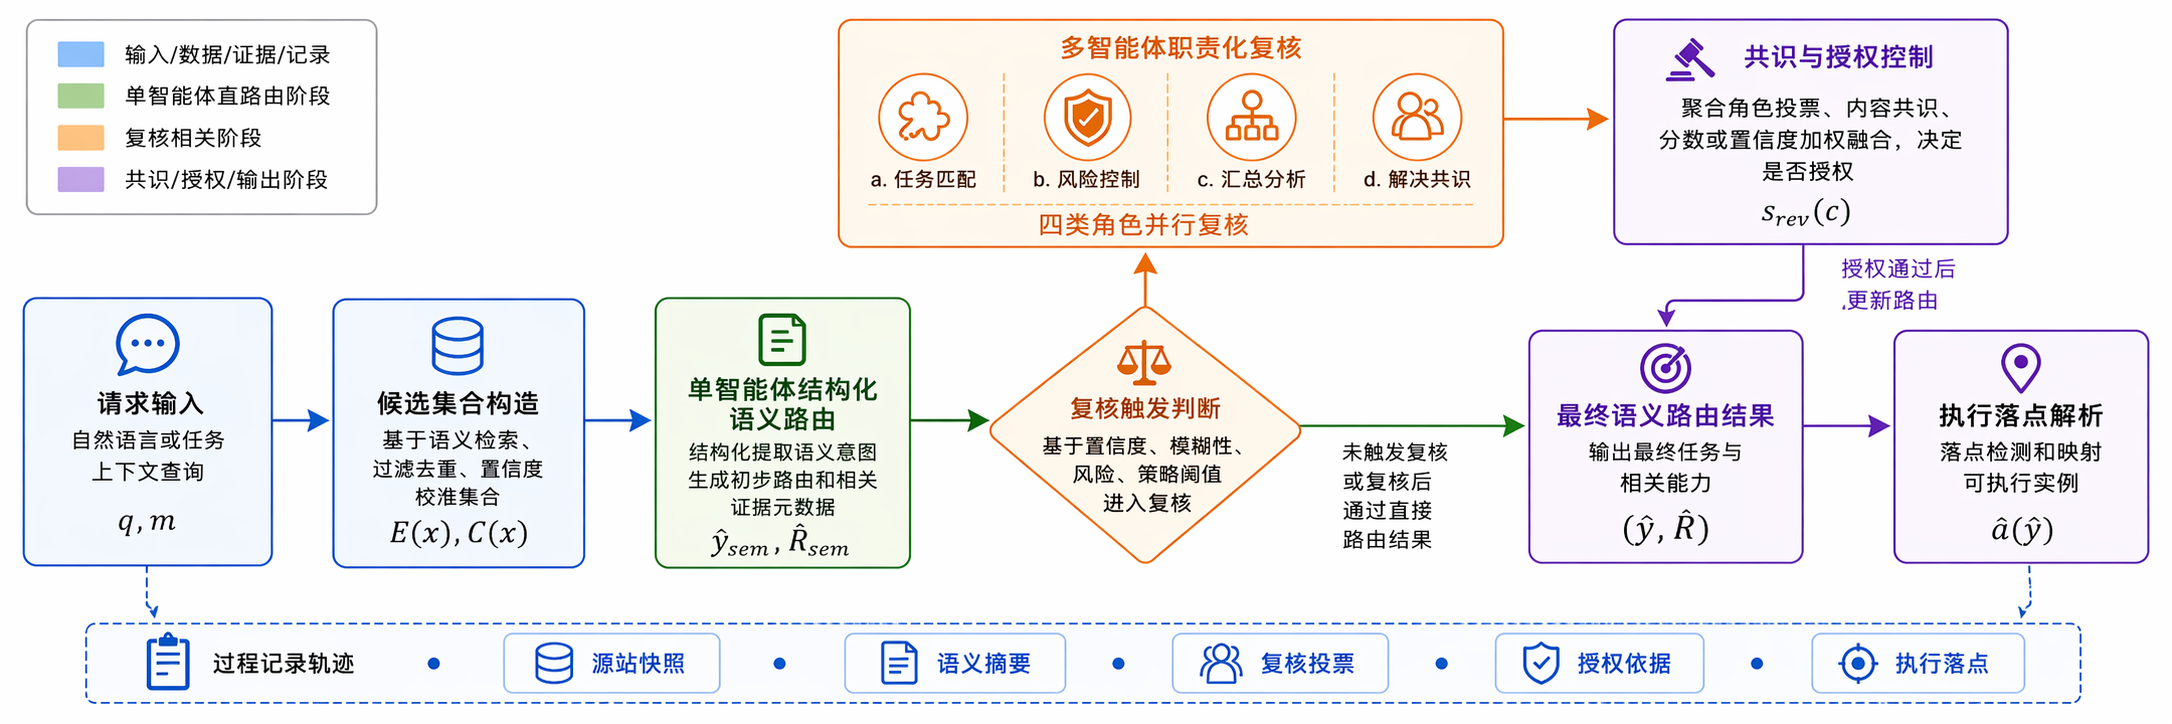
\includegraphics[width=\textwidth]{figures/fig1_framework.png}
\caption{单智能体与多智能体协同语义路由方法流程。系统首先构造候选集合并限定搜索边界；结构化语义路由在候选集合内部完成主能力判断与相关能力识别；职责化协作复核按触发条件启动，并通过显式授权控制改判边界。}
\label{fig:framework}
\end{figure*}

\subsection{候选集合构造与规则基线}

系统首先依据节点描述、别名、层级信息与元数据标签构造候选集合，并将后续主能力判断和相关能力识别限制在该集合内部。候选集合构造阶段整合别名匹配、描述相似度、上下文命中和层级关系等确定性信号，形成 top-$K$ 候选列表及其候选优先级。统一候选边界使不同路由策略能够在同一候选空间内比较判别效果，并减少下游语义判别信号对候选集合构造过程的前置影响。

在此基础上，规则基线路由计算候选级主任务分数
\begin{equation}
\begin{aligned}
s_{\mathrm{rule}}(c\mid x)=\;&\omega_r \tilde s_C(c)+\omega_p \phi_{\mathrm{pri}}(c)+\omega_c \phi_{\mathrm{ctx}}(c)\\
&+\omega_h \phi_{\mathrm{hier}}(c)+\omega_s \phi_{\mathrm{spec}}(c)-\Pi_{\mathrm{struct}}(c),
\end{aligned}
\end{equation}
其中 $\tilde s_C(c)$ 表示候选集合构造阶段形成的候选优先级，$\phi_{\mathrm{pri}}$、$\phi_{\mathrm{ctx}}$、$\phi_{\mathrm{hier}}$ 和 $\phi_{\mathrm{spec}}$ 分别表示主任务命中、上下文匹配、层级支持和粒度适配信号，$\Pi_{\mathrm{struct}}$ 为结构性惩罚项。规则路由提供可解释基线，也为后续的结构化语义判别提供稳定的融合底座。

结合当前实现，规则基线的候选级信号主要由别名匹配、描述相似度、上下文命中、层级关系、一致性证据和节点类型适配共同组成；结构性惩罚则主要针对父节点过粗、仅命中次要诉求、仅命中场景描述的子节点误命中以及回退节点误用等情况设置。直接路由阶段固定保留 top-\texttt{5} 候选用于主能力和相关能力排序；单智能体语义判别阶段进一步从候选快照中截取 top-\texttt{8} 候选构造结构化裁决包，以便在固定边界内完成更充分的候选比较。

\subsection{结构化语义判别}

结构化语义判别是本文提高路由准确率的关键环节。该模块读取 top-$K$ 候选说明包，返回受约束的结构化字段，包括主能力候选、相关能力候选、任务匹配度、主能力匹配度、相关能力匹配度、粒度判断、风险失配标记以及语义交接信息。候选说明包中除候选名称与描述外，还包含场景摘要、主任务摘要、次要诉求、竞争候选说明和初始规则分数，用于帮助模型在固定候选边界内完成稳定比较。其输出写为
\begin{equation}
z_{\mathrm{sem}}(x)=\bigl(\hat y_{\mathrm{sem}},\hat R_{\mathrm{sem}},s_{\mathrm{sem}},H(x),J(x)\bigr),
\end{equation}
其中 $H(x)$ 编码场景摘要、主任务摘要、不确定性摘要和混淆点，$J(x)$ 表示候选级结构化判断表。

随后，系统将规则分数与结构化语义判断进行候选内融合：
\begin{equation}
\begin{aligned}
s_{\mathrm{sem}}(c\mid x)=\;&\alpha_1 \widetilde s_{\mathrm{rule}}(c)
+\alpha_2 \widetilde s_C(c)
+\alpha_3 f_{\mathrm{task}}(c)\\
&+\alpha_4 f_{\mathrm{pri}}(c)
+b_{\mathrm{sel}}(c)
-\delta_{\mathrm{risk}}(c),
\end{aligned}
\end{equation}
其中 $\widetilde s_{\mathrm{rule}}$ 为规则主路由分数归一化结果，$\widetilde s_C(c)$ 为候选集合构造阶段候选优先级的归一化结果，$f_{\mathrm{task}}$ 和 $f_{\mathrm{pri}}$ 分别对应结构化输出中的任务匹配度和主能力匹配度，$b_{\mathrm{sel}}$ 奖励被显式选为主能力的候选，$\delta_{\mathrm{risk}}$ 表示风险失配惩罚。该步骤不仅提高了候选集合内部的区分能力，也为后续协作复核提供了可直接使用的语义摘要、竞争候选说明和不确定性来源。当前实现中，该阶段采用 \texttt{deepseek-chat} 模型，以结构化 JSON 方式输出裁决包，从而提升结果可复核性。

当前结构化裁决包中除候选列表和规则分数外，还包含场景摘要、主次意图摘要、候选级裁决表、混淆点以及主要竞争候选说明等结构化字段。系统要求主能力和相关能力输出均来自当前候选集合，并将相关能力输出上限控制为 3 个。当前实现采用温度为 0 的结构化输出方式，\texttt{max\_tokens} 设为 1800；当直接路由置信度低于 0.62、top-1 与竞争候选间隔低于 0.08、高风险样本分数间隔低于 0.14，或模型主动请求升级时，样本将被标记进入协作复核阶段。

\subsection{职责化协作复核}

职责化协作复核用于处理低置信、置信间隔过小、高风险和多意图冲突样本。与开放式多智能体讨论不同，本文始终将协作模块限制在固定候选集合内部，并通过职责分工约束每个角色的可见证据与判断范围。本文采用四类职责角色：任务匹配角色负责任务识别，治理风险角色负责风险边界审查，层级解析角色负责父子层级与粒度冲突判别，用户偏好角色负责主次意图拆分与偏好线索提取。四个角色共享同一候选集合，但只读取与本职责相关的证据视图，并在统一控制器下完成聚合。

\begin{table}[htbp]
\centering
\caption{职责化协作复核中的角色分工}
\label{tab:roles}
\small
\begin{tabularx}{\columnwidth}{lYY}
\toprule
角色 & 关注证据 & 主要职责 \\
\midrule
任务匹配角色 & 主诉求短语、候选描述、显式主任务证据 & 判断哪个候选最能直接承接主任务 \\
治理风险角色 & 风险标签、跨域竞争关系、负向证据 & 审查高风险节点与跨域改判是否成立 \\
层级解析角色 & 父子链、同层竞争、粒度适配信号 & 处理父子节点、同层级节点之间的粒度冲突 \\
用户偏好角色 & 次要诉求、相关能力候选、主次意图线索 & 区分主任务与次任务，辅助相关能力识别 \\
\bottomrule
\end{tabularx}
\end{table}

对每个角色 $r\in\mathcal R$，系统构造角色专属视图
\begin{equation}
P_r(x)=\Pi_r\bigl(E(x),z_{\mathrm{sem}}(x),H(x)\bigr),
\end{equation}
并输出角色提案
\begin{equation}
o_r(x)=\bigl(\hat y_r,\hat R_r,\rho_r,\kappa_r,\sigma_r\bigr),
\end{equation}
其中 $\rho_r$ 为角色置信度，$\kappa_r$ 表示是否支持改判，$\sigma_r$ 为职责维度上的支持/阻止/中性信号。控制器在第一轮聚合角色提案后，计算候选级复核分数
\begin{equation}
\begin{aligned}
s_{\mathrm{rev}}^{(1)}(c\mid x)=\;&0.40\,v(c)
+0.25\,\bar{\rho}(c)
+0.15\,s_{\mathrm{sem}}(c)\\
&+0.10\,e(c)
+0.10\,r(c)
+\varsigma(c).
\end{aligned}
\end{equation}
其中 $v(c)$ 表示把候选 $c$ 作为主能力的角色比例，$\bar{\rho}(c)$ 表示相应角色的平均置信度，$e(c)$ 表示显式证据强度，$r(c)$ 表示相关能力投票比例，$\varsigma(c)$ 表示职责信号的带符号加权和。若第一轮排序前两名之间的差距过小，或第一名相对直接路由结果构成敏感改判，则系统进一步触发第二轮复核。第二轮围绕当前候选与挑战候选进行定向比较，并保持原有候选空间约束。

显式授权机制控制协作复核的最终改判。若复核结果相对直接路由结果构成改判，则系统要求同时满足：足够的改判支持票数、足够的共识分数增益和足够强的显式主任务证据；对于高风险、跨层级或跨域改判，还要求第二轮共识和相应职责角色的责任确认。由此，复核触发和最终改判分别受独立条件控制。

当前实现中，异构协作模式使用 4 个职责角色并行复核；单角色模式只保留通用复核角色；同质复核模式则复制通用复核角色 4 次以构造对照实验。不同角色读取的候选视图规模上限均为 5，并共享同一直接路由阶段语义摘要，但在可见字段、关注候选和温度设置上保持差异，从而尽可能提高职责互补性。

\subsection{协作触发与改判授权}

协作复核采用显式条件触发策略。根据当前实现，直接路由结果满足下列条件之一时进入职责化复核流程：1）主能力置信度低于阈值；2）top-1 与 top-2 间隔过小；3）结构化语义判别阶段主动请求复核；4）当前主能力属于高风险节点，且分数间隔不足或存在治理回退信号；5）样本存在多意图迹象但相关能力未被稳定识别。其余样本保留结构化语义路由结果。该设置将额外判断资源集中用于高风险、高歧义样本，从而兼顾复杂样本修正需求与整体处理效率。

协作结果改变直接路由结果时，还需通过显式授权规则。当前实现要求候选改判结果同时满足：1）达到最小改判票数；2）最终共识分数相对直接路由结果有足够增益；3）具有足够强的显式主任务证据。对于高风险改判、跨层级改判和跨域改判，系统还要求第二轮复核共识以及更强的显式证据支持。授权条件外的样本保留结构化语义路由结果。

本文比较的默认配置、选择性配置和扩展配置，对应不同的复核触发范围和改判门槛。默认配置采用高精度授权策略，选择性配置扩大高价值复杂样本的协作覆盖，扩展配置进一步利用协作复核证据并覆盖更多高价值改判机会。这样的设置便于在实验中比较不同协作强度下的结果差异。
职责化协作复核的具体处理流程如图\ref{fig:flow} 所示。

\begin{figure*}[htbp]
\centering
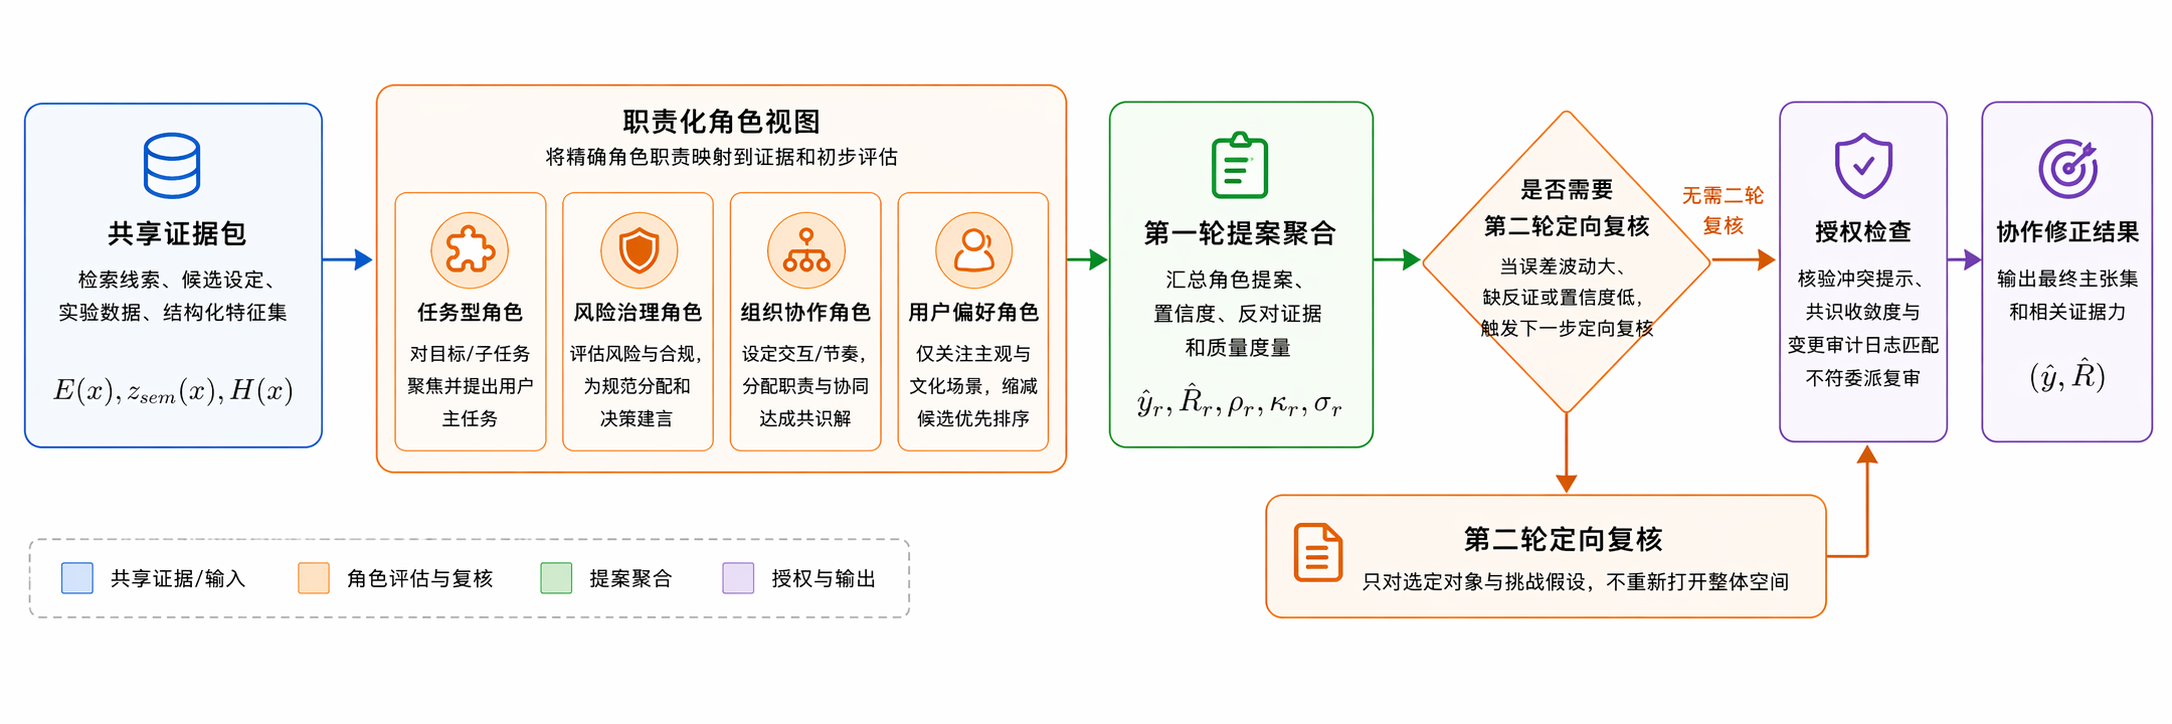
\includegraphics[width=\textwidth]{figures/fig2_review_flow.png}
\caption{职责化协作复核流程。系统先聚合多角色提案，再按需要触发第 2 轮定向复核，并在最终改判前执行授权检查。}
\label{fig:flow}
\end{figure*}

\subsection{过程记录与执行接口}

为支持样本级审计，本文为每个样本记录统一过程轨迹：
\begin{equation}
\begin{aligned}
T(x)=\bigl(&E(x), z_{\mathrm{rule}}(x), z_{\mathrm{sem}}(x), g(x),\\
&\{o_r(x)\}_{r\in\mathcal{R}}, z_{\mathrm{rev}}(x), \hat a(x)\bigr).
\end{aligned}
\end{equation}
其中包含候选快照、直接路由输出、升级信号、角色提案、角色可见视图、复核聚合结果、改判来源和执行接口信息。该过程记录既用于样本级错误定位，也用于分析协作复核发挥净修正作用的触发条件。

执行接口模块则在给定主能力地址的前提下，在实例集合 $A(\hat y)$ 中完成可执行实例选择，并保持上游语义路由结论稳定。当前实现坚持四项约束：接受与主能力地址精确匹配的实例；在执行层保持能力地址一致；实例选择采用确定性评分；对离线、缺失 endpoint 或 schema 不兼容实例进行硬过滤。在此基础上，系统采用由语义匹配、schema 兼容、服务标签、健康度和公平曝光组成的可解释评分函数，对候选实例排序：
\begin{equation}
\begin{aligned}
\text{final}(a)=\;&\text{base}(a)\cdot \text{health}(a)\\
&\cdot \text{fair}_{\text{agent}}(a)\cdot \text{fair}_{\text{provider}}(a),
\end{aligned}
\end{equation}
其中
\begin{equation}
\begin{aligned}
\text{base}(a)=\;&0.55\,S_{\text{match}}(a)\\
&+0.25\,S_{\text{schema}}(a)+0.20\,S_{\text{tag}}(a).
\end{aligned}
\end{equation}
该环节作为系统输出接口保留在方法框架中，使语义路由结果能够继续接入实际服务调用链路。

\section{实验设置}

\subsection{数据与评测协议}

为检验所提方法在受限能力命名空间语义路由问题上的有效性，本文围绕预先定义的能力命名空间整理得到总计 \texttt{563} 条真实样本，并冻结划分为统一的 \texttt{train=450} 和 \texttt{test=113}。训练划分用于提示词形式、触发阈值、改判授权门槛和协作决策配置的开发与冻结；测试划分用于在固定配置下评估方法效果。正文报告训练集与测试集两侧结果，其中训练侧结果用于呈现配置选择依据和机制一致性，测试侧结果用于检验冻结配置下的最终表现。

数据标签围绕方法验证目标展开，主标签记为 \texttt{ground\_truth\_fqdn}，同时设置 \texttt{acceptable\_fqdns} 和 \texttt{relevant\_fqdns} 两类辅助标注，以分别覆盖层级合理回落和相关能力识别现象。这一标注方式用于验证三个核心能力：主能力是否选对、层级合理回落是否可接受、相关能力是否识别充分。

\begin{table}[htbp]
\centering
\caption{样本标注字段说明}
\label{tab:labels}
\small
\begin{tabularx}{\columnwidth}{lY}
\toprule
字段 & 含义与用途 \\
\midrule
\texttt{ground\_truth\_fqdn} & 主能力标准答案，用于统计主标签准确率 \\
\texttt{acceptable\_fqdns} & 可接受主标签集合，用于覆盖层级合理回落或等价入口情形 \\
\texttt{relevant\_fqdns} & 相关能力集合，用于统计相关能力召回率与精确率 \\
\bottomrule
\end{tabularx}
\end{table}

\begin{table}[htbp]
\centering
\caption{数据集与命名空间画像}
\label{tab:profile}
\small
\begin{tabularx}{\columnwidth}{lY}
\toprule
指标 & 统计值 \\
\midrule
样本总数 & \texttt{563}（训练集 \texttt{450}，测试集 \texttt{113}） \\
样本覆盖主标签种类 & \texttt{45} 类 \\
命名空间节点总数 & \texttt{50} 个（一级能力域 \texttt{9} 个，二级能力域 \texttt{24} 个） \\
测试集 top-\texttt{8} 候选包 gold 覆盖率 & \texttt{97.35\%}（\texttt{110/113}） \\
测试集含相关能力标注样本占比 & \texttt{33.63\%}（\texttt{38/113}） \\
测试集多意图/高风险样本数 & \texttt{12} / \texttt{4} \\
\bottomrule
\end{tabularx}
\end{table}

表\ref{tab:profile} 给出了统一评测集的基本画像。本文任务属于 \texttt{50} 个节点组成的受限能力命名空间内的主能力与相关能力判断问题；测试集保留了一定比例的相关能力样本、多意图样本和高风险样本，用于检验方法在复杂边界情形下的稳定性。

目前公开工具调用和函数调用基准主要集中在 API 调用生成、工具增强对话和函数调用执行评价上，尚未覆盖本文所关注的“自然语言请求到受限能力命名空间能力地址”的同口径语义路由任务。表\ref{tab:neighbor_datasets} 给出了相邻公开基准与本文评测集的关系。本文数据集规模与 API-Bank 等人工标注评测基准处于同一量级，高于其人工工具使用对话数；同时显著小于 ToolBench 这类自动构造的大规模工具学习数据。因此，本文 \texttt{563} 条样本更接近面向新子任务的小规模高质量验证集，而非通用工具调用训练集。

\begin{table*}[htbp]
\centering
\caption{相邻公开基准与本文数据集的关系}
\label{tab:neighbor_datasets}
\small
\setlength{\tabcolsep}{5pt}
\begin{tabularx}{0.96\textwidth}{p{2.8cm}p{4.0cm}Y}
\toprule
数据集/基准 & 规模与评测对象 & 与本文任务的关系 \\
\midrule
API-Bank\cite{apibank} & 73 个 API 工具，314 段人工工具使用对话，753 次 API 调用；另含 1888 段训练对话 & 关注工具增强对话中的规划、检索和调用能力；与本文同属工具调用前后链路，但不评估受限命名空间内的能力地址路由 \\
ToolBench\cite{toollm} & 3451 个工具、16464 个 API、126486 条实例，主要由自动流程生成和过滤 & 面向开放域真实 API 的大规模工具学习与检索调用；规模远大于本文，但数据构建方式和目标任务不同 \\
Gorilla\cite{gorilla} & 覆盖 1600 余个 API 调用，强调自然语言到 API 调用表达的正确生成 & 关注 API 调用语义和语法正确性；本文更关注执行前的能力地址选择、层级回落和相关能力识别 \\
BFCL\cite{bfcl} & 面向真实函数调用场景的函数选择、参数生成和多函数调用评测 & 关注函数调用执行评价；可作为函数调用能力评测参照，但不覆盖本文的命名空间路由和职责化复核机制 \\
本文数据集 & 563 条真实样本，受限能力命名空间 50 个节点，冻结划分为 train=450、test=113 & 面向受限能力命名空间语义路由构建，评估主能力选择、可接受回落、相关能力识别和协作复核净修正 \\
\bottomrule
\end{tabularx}
\end{table*}

为进一步刻画方法作用机制，本文开展两类分析：一类是训练集确定决策配置后在同一冻结测试集上的固定配置比较，用于观察协作复核在不同触发范围和授权门槛下的收益变化；另一类是后验诊断和协作消融，用于刻画修正主要出现在哪些样本类型和协作协议上。两类分析与统一主协议结果相互印证，使性能提升、触发范围和样本属性之间的关系更加清晰。
数据与评测协议如图\ref{fig:protocol} 所示。

\begin{figure}[htbp]
\centering
\resizebox{0.94\columnwidth}{!}{%
\begin{tikzpicture}[paper diagram, node distance=0.82cm and 0.95cm]
\node[tracebox, text width=2.8cm] (pool) {统一样本集\\\textbf{563 条}};
\node[bluebox, below left=0.95cm and 1.0cm of pool, text width=2.2cm] (train) {训练集\\\textbf{450}};
\node[accentbox, below right=0.95cm and 1.0cm of pool, text width=2.2cm] (test) {测试集\\\textbf{113}};
\node[tealbox, below=0.9cm of train, text width=3.8cm] (develop) {训练阶段用途\\提示词、阈值、授权策略与配置开发};
\node[warmbox, below=0.9cm of test, text width=3.8cm] (report) {测试阶段用途\\主结果报告、诊断分析、协作消融};
\draw[flowarrow] (pool) -- (train);
\draw[flowarrow] (pool) -- (test);
\draw[flowarrow] (train) -- (develop);
\draw[flowarrow] (test) -- (report);
\end{tikzpicture}
}
\caption{数据与评测协议。本文围绕受限能力命名空间语义路由方法构建 \texttt{563} 条样本的统一 \texttt{train/test} 主协议；训练划分用于配置开发与冻结，测试划分用于固定配置评估，后验诊断和协作消融用于呈现复杂样本中的收益分布。}
\label{fig:protocol}
\end{figure}

\subsection{评测指标}

系统主要报告四类指标。第一，主标签准确率衡量主能力是否被正确选出。第二，可接受主标签准确率允许命中预定义的等价标签，用于覆盖层级合理回落的情况。第三，相关能力召回率与精确率用于评估辅助能力识别的完整性和准确性。第四，系统额外记录改判/纠错/误改诊断指标，用于分析协作复核的净修正收益。

其中，“改判”表示协作复核路径相对于参考路径改变了多少个样本的主预测；“纠错”表示这些改判中有多少个把原本错误的样本修正为正确；“误改”表示其中有多少个把原本正确的样本改为错误结果。统一主结果和协作消融以对应的单智能体或规则路由结果为参考，配置比较以默认配置为参考。该指标与准确率共同刻画协作复核带来的净收益和改判质量。

本文从四个层面报告实验结果：统一 \texttt{train/test} 主协议用于给出整体性能；累计样本池稳定性分析用于观察样本规模扩展下的方法排序变化；后验诊断分析用于解释收益主要出现在哪些类型样本上；协作消融用于分析多智能体协作在不同协议下的有效性。

\subsection{对比系统与实验配置}

具体比较对象包括 4 组系统。1）规则路由基线：只使用候选集合构造与规则主分数完成主能力判断和相关能力识别。2）规则路由基线加协作复核：在规则路由结果上追加职责化协作复核。3）单智能体结构化语义路由基线：在相同候选集合内使用大模型结构化判别与分数融合作为主路由结果。4）单智能体结构化语义路由加协作复核：在单智能体结果基础上追加职责化协作复核。上述对比系统共用相同的命名空间、候选集合和评测协议，从而确保性能差异主要来自语义判别与复核策略本身。

实验中，单智能体结构化语义路由、相关能力识别与多智能体协作复核均采用 \texttt{deepseek-chat} 模型实现，规则路由基线为非大模型确定性方法。单智能体阶段采用温度为 0 的结构化 JSON 输出，以降低结果波动；多智能体阶段依据不同职责角色采用中低温解码参数，其中任务匹配角色温度为 0.50，治理风险角色为 0.20，层级解析角色为 0.35，用户偏好角色为 0.70。协作模块默认最多运行两轮：第一轮用于多角色并行提案，第二轮只在当前候选与挑战候选差距过小或涉及敏感改判时触发。

\begin{table}[htbp]
\centering
\caption{关键实验参数设置}
\label{tab:params}
\small
\begin{tabularx}{\columnwidth}{lY}
\toprule
参数项 & 设置值 \\
\midrule
候选说明包规模 & 单智能体阶段输入 top-\texttt{8} 候选，直接路由结果保留 top-\texttt{5} \\
相关能力上限 & 单智能体阶段最多输出 \texttt{3} 个相关能力 \\
单智能体解码参数 & \texttt{temperature=0.0}，\texttt{max\_tokens=1800} \\
协作角色数量 & 异构模式下共 4 个角色，分别承担任务匹配、治理风险、层级解析和用户偏好复核 \\
协作轮数 & 最多 2 轮，第 2 轮在候选间隔不足或涉及敏感改判时触发 \\
协作解码参数 & 角色温度分别为 0.50、0.20、0.35 和 0.70，\texttt{max\_tokens=3000} \\
改判授权阈值 & 最少 \texttt{3} 票支持，分数增益不少于 \texttt{0.08}，显式主任务证据不少于 \texttt{0.55} \\
\bottomrule
\end{tabularx}
\end{table}

本文进一步比较三种协作决策配置：默认配置、选择性配置和扩展配置。三种配置的触发阈值和改判门槛均在训练集上完成开发并冻结，测试集用于固定配置结果报告。默认配置和选择性配置采用较高复核触发阈值与改判门槛，扩展配置则更充分利用协作复核证据并覆盖更多高价值改判机会。该设置将复核触发范围与改判授权门槛分离，便于观察协作链路在不同决策强度下的作用。

\section{实验结果与分析}

\subsection{统一主结果}

统一 \texttt{train/test} 主协议下的结果如表\ref{tab:main} 所示。

\begin{table*}[htbp]
\centering
\caption{统一 \texttt{train/test} 主协议下的主标签结果}
\label{tab:main}
\small
\setlength{\tabcolsep}{3.8pt}
\resizebox{\textwidth}{!}{%
\begin{tabular}{lccccc}
\toprule
系统 & 训练集主准确率 & 训练集改判/纠错/误改 & 测试集主准确率 & 测试集可接受准确率 & 测试集改判/纠错/误改 \\
\midrule
规则路由基线 & 0.8156 & -- & 0.7876 & 0.8142 & -- \\
规则路由基线 + 协作复核 & 0.8244 & 5 / 4 / 1 & 0.8053 & 0.8319 & 2 / 2 / 0 \\
单智能体结构化语义路由基线 & 0.8756 & -- & 0.8761 & 0.9027 & -- \\
单智能体结构化语义路由 + 协作复核 & 0.8844 & 4 / 4 / 0 & 0.8850 & 0.9115 & 1 / 1 / 0 \\
\bottomrule
\end{tabular}
}
\end{table*}

表\ref{tab:main} 显示，单智能体结构化语义路由在统一主协议下形成了稳定增益。训练集上，主标签准确率由规则路由基线的 0.8156 提升到 0.8756，加入默认协作复核后达到 0.8844，并取得 \texttt{4/4/0} 的改判/纠错/误改结果。测试集上，单智能体结构化语义路由将主标签准确率从 0.7876 提升到 0.8761，将可接受主标签准确率从 0.8142 提升到 0.9027；在此基础上加入默认协作复核后，系统主标签准确率进一步达到 0.8850，并保持零误改。

上述提升呈现出清晰的分层特征。规则路由基线能够在语义明确、层级关系简单的样本上给出稳定结果，但在跨域重叠、父子节点冲突和多意图请求中，候选内区分能力仍然有限。引入单智能体结构化语义路由后，系统能够在固定候选边界内显式比较主任务匹配度、粒度适配程度和风险失配信号，主标签准确率和可接受准确率因而同步提升。有限候选空间内的语义判别能力，是协同路由框架取得稳定收益的基础。

默认协作复核在训练集和测试集上均体现出高精度授权特征：训练侧 4 次主标签改判均形成纠错，测试侧共有 \texttt{50/113}（\texttt{44.25\%}）个样本进入协作复核，其中 1 个样本发生主标签改判并被有效修正。该结果说明，协作链路能够在边界样本上提供受控修正，并与前序结构化语义判别形成互补。

\begin{table}[htbp]
\centering
\caption{统一 \texttt{train/test} 主协议下的相关能力识别结果}
\label{tab:related}
\resizebox{\columnwidth}{!}{%
\begin{tabular}{lcccc}
\toprule
系统 & 训练集相关召回率 & 训练集相关精确率 & 测试集相关召回率 & 测试集相关精确率 \\
\midrule
规则路由基线 & 0.2822 & 0.3833 & 0.2895 & 0.3793 \\
单智能体结构化语义路由基线 & 0.3129 & 0.4080 & 0.3684 & 0.4242 \\
\bottomrule
\end{tabular}
}
\end{table}

相关能力识别结果如表\ref{tab:related} 所示。该指标以直接路由阶段为主要统计对象。与规则路由基线相比，单智能体结构化语义路由基线将测试集相关能力召回率从 0.2895 提升到 0.3684，相关能力精确率从 0.3793 提升到 0.4242。

相关能力识别指标从辅助任务角度呈现出一致趋势。主能力判断提升的同时，相关能力召回率和精确率也同步提高，表明结构化语义判别不仅改善主能力选择，也增强了对辅助能力和关联能力的识别能力。当模型能够在候选集合内部更准确地区分主次任务关系时，相关能力集合的构造也更加完整和稳定。

默认协作复核在相关能力识别指标上延续了结构化语义判别阶段形成的稳定表现。结合当前触发条件和优化目标可见，两阶段框架形成了明确分工：结构化语义判别负责主次任务摘要和候选级证据构造，协作复核负责在主能力不确定样本上引入职责化复核视角。该分工使主能力判断和相关能力识别在同一候选证据基础上得到同步提升。
统一主结果与扩展决策配置结果之间的增益关系如图\ref{fig:waterfall} 所示。

\begin{figure}[htbp]
\centering
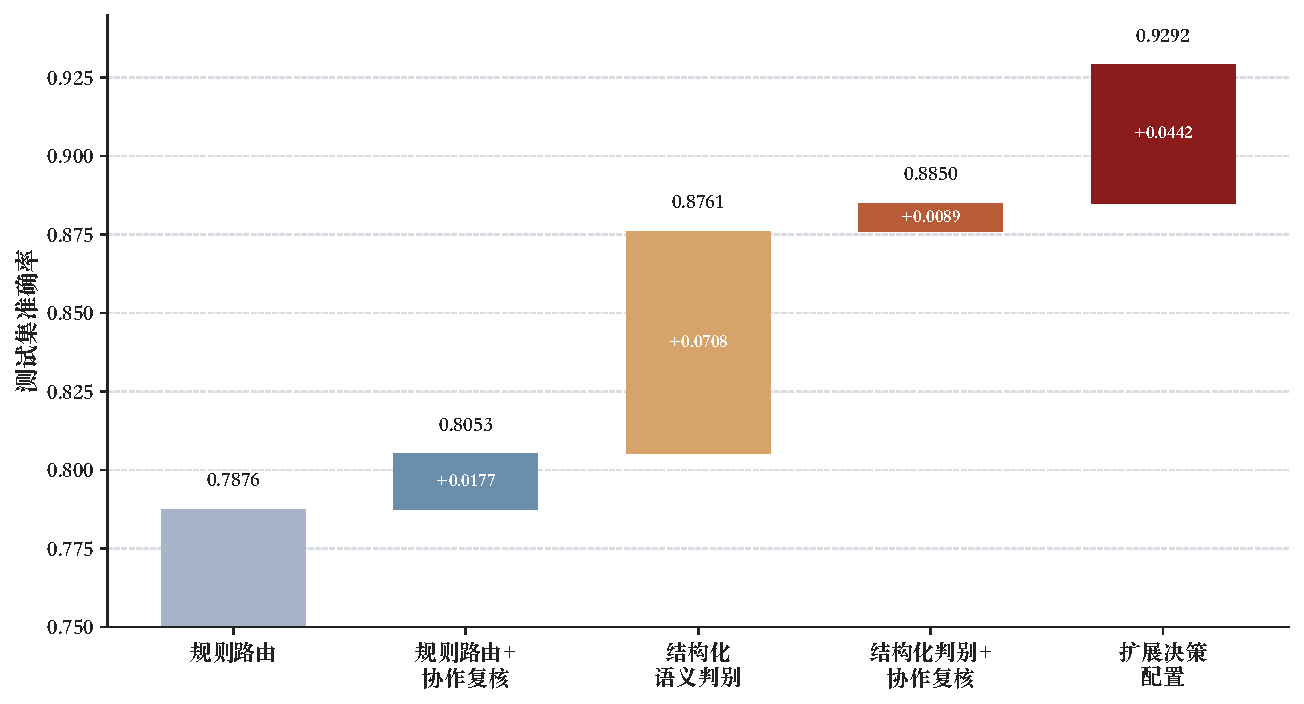
\includegraphics[width=\columnwidth]{figures/01_pooled_test_waterfall.pdf}
\caption{统一主结果与扩展决策配置结果的增益对比图}
\label{fig:waterfall}
\end{figure}

\subsection{扩展决策配置分析：协作何时有效}

三种在训练集上确定并冻结的协作决策配置结果见表\ref{tab:config}。该表使用统一评测集的训练侧 \texttt{450} 条样本和测试侧 \texttt{113} 条样本，用于报告默认配置、选择性配置和扩展配置在统一主协议下的整体表现。

\begin{table}[htbp]
\centering
\caption{不同协作决策配置的训练集与测试集结果（训练侧 \texttt{n=450}，测试侧 \texttt{n=113}）。测试集改判/纠错/误改相对于默认配置统计。}
\label{tab:config}
\resizebox{\columnwidth}{!}{%
\begin{tabular}{lcccc}
\toprule
配置 & 训练集准确率 & 测试集准确率 & 测试集改判/纠错/误改 & 测试集增量 \\
\midrule
默认配置 & 0.8800 & 0.8850 & -- & 0.0000 \\
选择性配置 & 0.8911 & 0.8938 & 1 / 1 / 0 & +0.0088 \\
扩展配置 & 0.8978 & 0.9292 & 5 / 5 / 0 & +0.0442 \\
\bottomrule
\end{tabular}
}
\end{table}

表\ref{tab:config} 报告三种冻结配置在训练集和测试集上的准确率变化。训练集比较中，默认配置、选择性配置和扩展配置的准确率分别为 0.8800、0.8911 和 0.8978，扩展配置在三种设置中取得最高结果。对应的测试结果保持同向排序，分别达到 0.8850、0.8938 和 0.9292；其中扩展配置相对默认配置提升 0.0442，并实现 \texttt{5/5/0} 的诊断结果，即 5 次改判均转化为有效纠错且没有引入误改。

表\ref{tab:config} 呈现了协作复核对决策配置的敏感性。训练侧比较用于确定不同触发范围和授权门槛下的配置选择；测试侧固定评估进一步显示，选择性配置和扩展配置均在默认配置基础上取得净收益，且没有出现误改。扩展配置在训练集和测试集上均保持最高准确率，表明当协作复核证据被更充分利用且改判授权规则保持约束时，协作复核可以形成更明显的净收益。

训练集与测试集上的同步趋势表明，协作触发和改判授权机制对结果改进具有稳定作用。结合改判/纠错/误改指标，扩展配置在测试侧表现为高质量改判。这一结果支撑了职责化协作复核作为复杂样本修正机制的有效性。不同协作决策配置在训练集和测试集上的对比如图\ref{fig:config} 所示。

\begin{figure}[htbp]
\centering
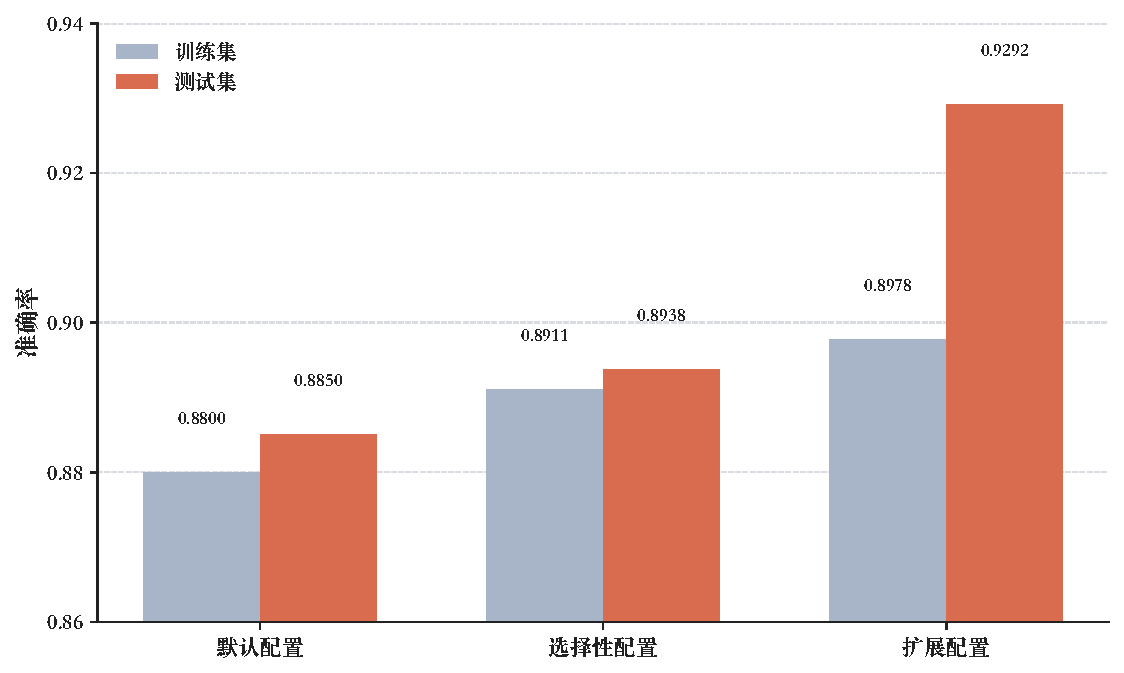
\includegraphics[width=\columnwidth]{figures/02_pooled_gate_selection.pdf}
\caption{不同协作决策配置的训练集与测试集结果}
\label{fig:config}
\end{figure}

\subsection{调用复杂度代理分析}

表\ref{tab:proxy} 给出了默认配置下的调用复杂度代理。该表以单智能体结构化语义路由作为每个请求的必经基线，统计默认协作复核带来的条件触发开销，用于呈现协作链路的工程成本特征。本文基于运行日志中稳定可得的过程记录，采用“调用当量 + 字符长度”的方式作为代理指标：前者刻画每个请求平均会额外触发多少次协作角色调用，后者刻画必经单智能体阶段和协作角色输出的大致文本规模。

\begin{table}[htbp]
\centering
\caption{默认配置的调用复杂度代理。单智能体结构化语义路由为必经基线，协作复核为条件触发增量。}
\label{tab:proxy}
\small
\begin{tabularx}{\columnwidth}{lYY}
\toprule
统计对象 & 指标 & 统计值 \\
\midrule
必经单智能体阶段 & 基础模型调用当量/请求 & \texttt{1.00} 次 \\
必经单智能体阶段 & 裁决包平均长度 & \texttt{5702} 字符 \\
必经单智能体阶段 & 结构化输出平均长度 & \texttt{3068} 字符 \\
默认协作增量 & 测试集进入协作复核样本占比 & \texttt{44.25\%}（\texttt{50/113}） \\
默认协作增量 & 进入协作样本的平均角色调用数 & \texttt{4.72} 次 \\
默认协作增量 & 进入协作样本的第二轮复核占比 & \texttt{18.00\%}（\texttt{9/50}） \\
默认协作增量 & 平均额外协作调用当量/请求 & \texttt{2.09} 次 \\
默认协作增量 & 协作角色单次输出平均长度 & \texttt{336} 字符 \\
默认配置总体 & 平均总模型调用当量/请求 & \texttt{3.09} 次 \\
\bottomrule
\end{tabularx}
\end{table}

表\ref{tab:proxy} 表明，单智能体结构化语义路由构成每个请求固定发生的基础调用；默认协作复核在 \texttt{44.25\%} 的测试样本上触发职责化复核。进入协作样本后，第二轮复核占比为 \texttt{18.00\%}，更高成本的二次讨论集中在少量边界情形。若以调用当量近似模型请求负载，则默认配置相对单智能体必经基线平均新增 \texttt{2.09} 次协作角色调用，总调用当量约为 \texttt{3.09} 次/请求。结合前述主结果可见，本文方法在保持协作链路受控触发的前提下，实现了复杂样本上的净修正收益。

扩展配置对应在训练集上确定后复用同一批协作复核过程记录所做的固定配置比较，其调用复杂度代理与表\ref{tab:proxy} 中的默认配置保持一致。\texttt{0.9292} 这一结果主要反映决策配置差异带来的净修正收益，模型调用开销与默认配置处于同一统计口径。

\subsection{样本池累计稳定性分析}

样本规模对结论稳定性的影响通过累计统计进行考察。本文基于既有逐样本预测结果，按照固定样本池顺序分别对训练划分和测试划分进行累计统计，结果如图\ref{fig:cumulative} 所示。该分析基于同一组模型、提示词和协作配置进行累计汇总；训练划分和测试划分分别计算，不进行合并统计。

累计趋势显示，小规模样本阶段的准确率受样本组成影响较大；随着累计样本数增加，结构化语义路由、默认协作复核和扩展配置的相对排序逐步稳定，且在后续样本加入后保持一致。测试划分在累计到 \texttt{73}、\texttt{93} 和 \texttt{113} 条样本时，结构化语义路由准确率分别为 \texttt{0.8767}、\texttt{0.8710} 和 \texttt{0.8761}，默认协作复核分别为 \texttt{0.8904}、\texttt{0.8817} 和 \texttt{0.8850}，扩展配置分别为 \texttt{0.9315}、\texttt{0.9355} 和 \texttt{0.9292}。新增样本主要扩展了任务覆盖和边界复杂度，核心方法相对规则基线的优势关系保持稳定。该趋势支持将当前 \texttt{563} 条训练/测试样本池作为本文方法比较的经验稳定验证基础。

\begin{figure*}[htbp]
\centering
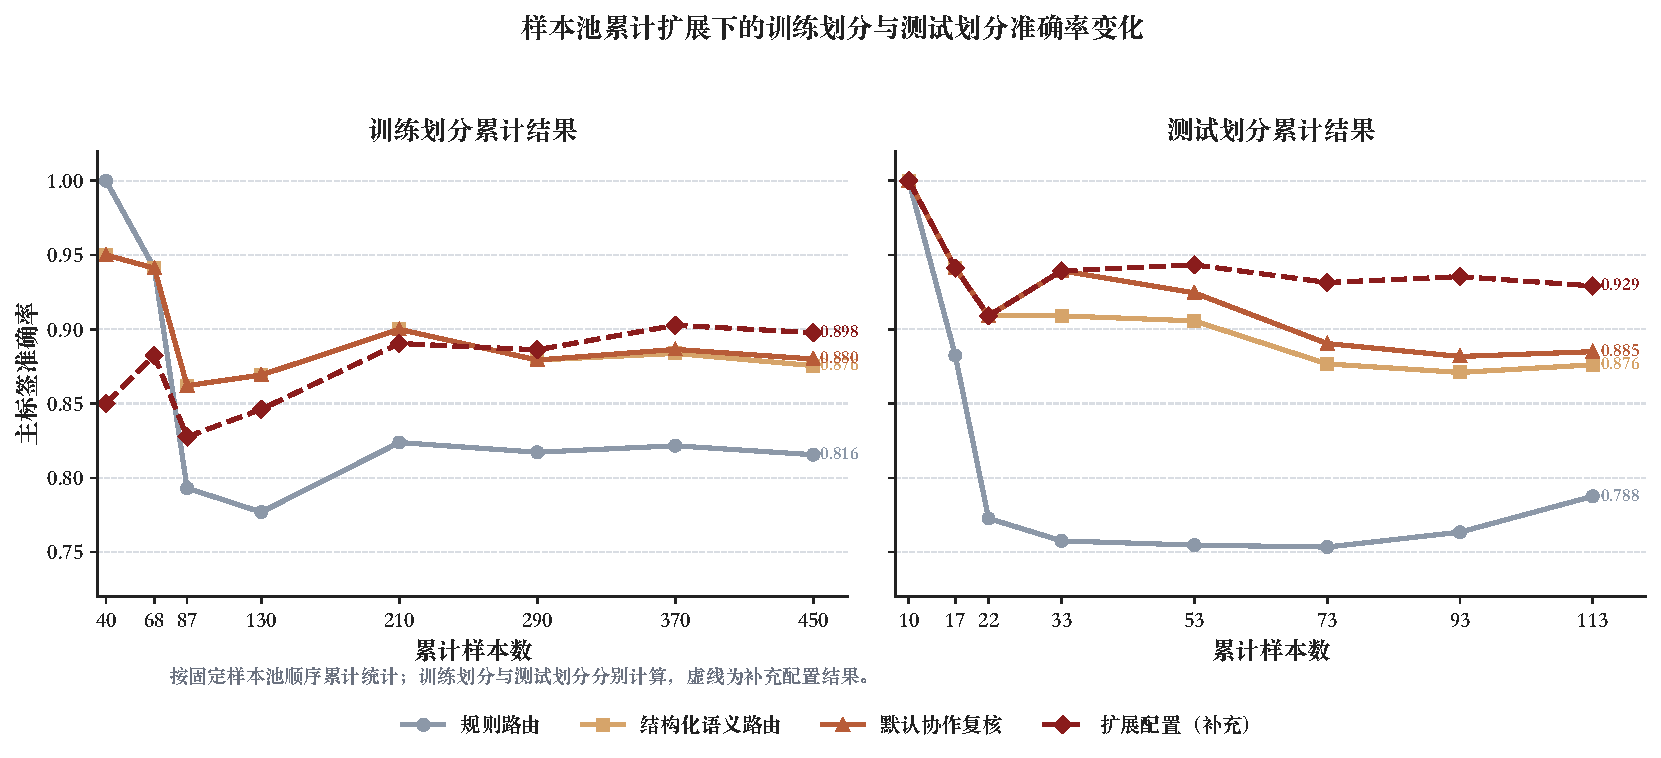
\includegraphics[width=\textwidth]{figures/09_historical_cumulative_train_test.pdf}
\caption{样本池累计扩展下的训练划分与测试划分准确率变化。训练划分和测试划分分别累计统计，横轴表示对应划分内的累计样本数；虚线表示扩展决策配置结果。图中呈现累计样本规模增加后方法排序和准确率区间的稳定性。}
\label{fig:cumulative}
\end{figure*}

\subsection{何种协作形式有效：协作复核消融}

不同协作协议之间的消融需要每个样本同时具备单角色复核、同质复核和职责化复核三类运行轨迹。基于这一配对比较要求，本文选取具备完整复核轨迹的样本构成配对消融样本集，其中训练侧包含 \texttt{320} 条样本，测试侧包含 \texttt{80} 条样本；样本进入该分析的条件是复核轨迹齐备，与预测正误无关。该样本集覆盖常规快路、层级竞争、主次意图拆分、跨域重叠和高风险治理等 5 类场景，用于在同一输入、同一候选空间和同一标注口径下比较不同协作协议的作用。在该样本集上，单智能体结构化语义路由基线的测试集准确率为 0.8625。表\ref{tab:ablation} 报告了单角色复核、同质复核和职责化协作复核三种设置下的结果。

\begin{table}[htbp]
\centering
\caption{配对消融样本集上的协作复核协议比较（训练侧 \texttt{n=320}，测试侧 \texttt{n=80}）。改判/纠错/误改相对于单智能体结构化语义路由基线统计。}
\label{tab:ablation}
\resizebox{\columnwidth}{!}{%
\begin{tabular}{lccccc}
\toprule
系统 & 训练集准确率 & 训练集改判/纠错/误改 & 测试集准确率 & 测试集增量 & 测试集改判/纠错/误改 \\
\midrule
单角色复核 & 0.8875 & 3 / 3 / 0 & 0.8625 & +0.0000 & 0 / 0 / 0 \\
同质复核 & 0.8844 & 2 / 2 / 0 & 0.8625 & +0.0000 & 0 / 0 / 0 \\
职责化协作复核（扩展配置） & 0.9187 & 13 / 13 / 0 & 0.9250 & +0.0625 & 5 / 5 / 0 \\
\bottomrule
\end{tabular}
}
\end{table}

表\ref{tab:ablation} 显示，训练侧不同协作协议已经呈现出明显差异。单角色复核和同质复核分别取得 \texttt{3/3/0} 与 \texttt{2/2/0} 的净纠错，职责化协作复核在扩展配置下达到 0.9187，并取得 \texttt{13/13/0} 的改判/纠错/误改结果。测试侧结果与训练侧趋势一致：单角色复核和同质复核保持在单智能体结构化语义路由基线水平，职责化协作复核与扩展配置配合时，系统准确率从 0.8625 提升到 0.9250，并实现 \texttt{5/5/0} 的净纠错。结果表明，职责化分工、结构化证据和改判控制的联合配置是形成协作收益的关键。

协作链路的有效性集中体现为三点：角色之间形成互补职责，复核过程围绕同一语义摘要开展定向比较，最终改判受到显式授权规则约束。职责化协作复核承担复杂样本上的条件化修正功能，与覆盖全量请求的直接路由阶段形成分工。不同协作协议在配对消融样本集上的结果对比如图\ref{fig:ablation} 所示。

\begin{figure}[htbp]
\centering
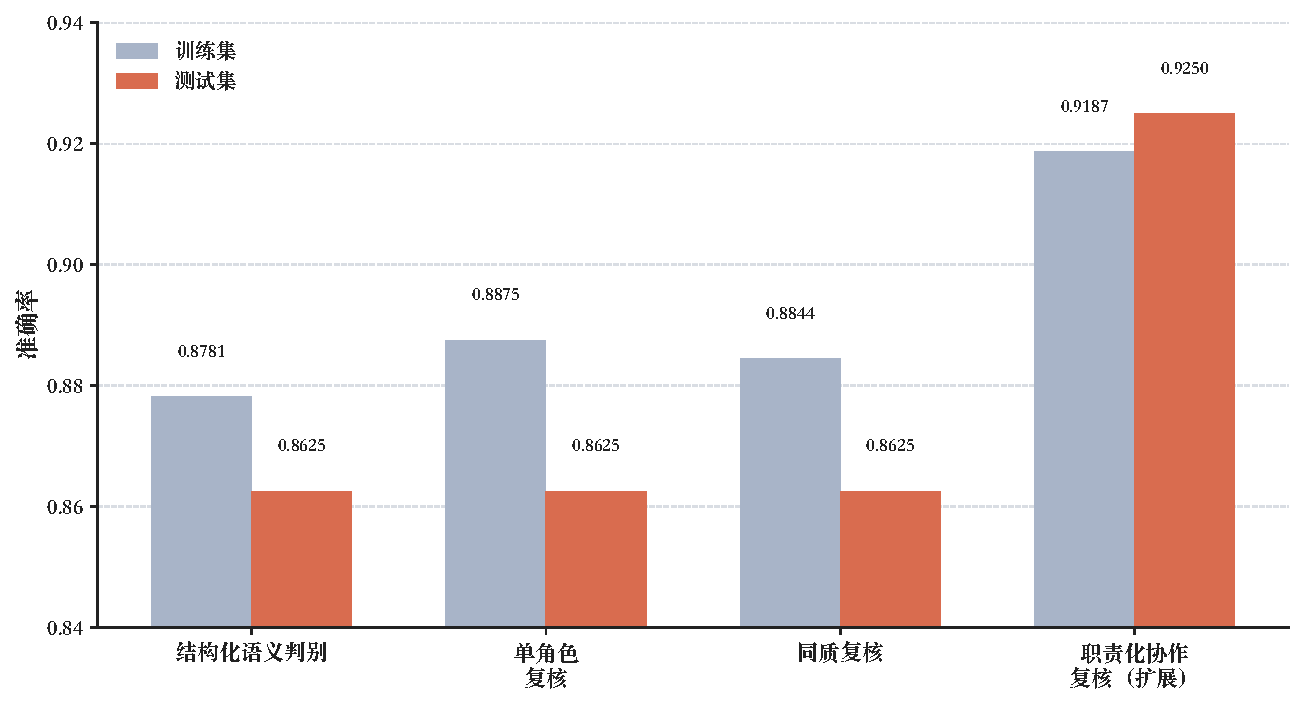
\includegraphics[width=\columnwidth]{figures/03_holdout3_collaboration_ablation.pdf}
\caption{配对消融样本集上的协作复核协议比较}
\label{fig:ablation}
\end{figure}

\subsection{后验诊断分析}

表\ref{tab:diag} 报告了 3 个后验诊断样本池上的结果。常规样本池主要包含语义明确、候选竞争较弱的请求；困难边界样本池主要包含跨域冲突、层级竞争和强歧义请求；扩展观察样本池主要包含命名空间覆盖范围扩展后更容易出现语义迁移和相关能力遗漏的请求。三者互斥，合计规模为 \texttt{113} 条，属于样本属性层面的结果分析，用于解释统一主协议结果中的收益来源。

\begin{table}[htbp]
\centering
\caption{后验诊断分析结果。各行对应统一样本集中的后验诊断样本池，用于分析不同样本属性下的收益分布。}
\label{tab:diag}
\resizebox{\columnwidth}{!}{%
\begin{tabular}{lccc}
\toprule
诊断样本池 & 样本数 & 单智能体结构化语义路由 & 单智能体结构化语义路由 + 协作复核 \\
\midrule
常规样本池 & 35 & 0.9143 & 0.9143 \\
困难边界样本池 & 24 & 0.6250 & 0.6667 \\
扩展观察样本池 & 54 & 0.8889 & 0.9074 \\
\bottomrule
\end{tabular}
}
\end{table}

后验诊断结果与主协议结论一致，并揭示了收益分布的主要来源。对于常规样本池，单智能体结构化语义路由已经达到较高水平，协作复核保持该水平；对于困难边界样本池，系统从 0.6250 提升到 0.6667；对于扩展观察样本池，系统从 0.8889 提升到 0.9074。

主协议中观察到的总体收益呈现明显的样本类型集中性，主要出现在语义重叠更强、层级冲突更明显或意图更混杂的样本池上。该现象与前述扩展决策配置分析以及配对消融样本集上的消融结果一致，表明协作复核主要承担复杂样本的二次甄别和净修正任务。

\subsection{典型样本分析}

表\ref{tab:cases} 列出配对消融样本集中的 3 个代表性案例，分别对应跨域竞争、多意图主次拆分和跨域重叠 3 类典型困难场景。

\begin{table*}[htbp]
\centering
\caption{配对消融样本集中的典型案例分析}
\label{tab:cases}
\small
\setlength{\tabcolsep}{4pt}
\begin{tabular}{p{1.8cm}p{1.9cm}p{5.4cm}p{5.6cm}}
\toprule
案例 & 现象类型 & 结果对比 & 修正原因 \\
\midrule
案例1 & 跨域竞争 & 内部编号：\texttt{000038}；真实主标签：\texttt{docs.productivity.cn}；单智能体结果：\texttt{course.education.cn}；协作结果：\texttt{docs.productivity.cn}。 & 词面命中将样本误拉向教育域，协作复核补充了文档处理证据与跨域比较后完成纠正。 \\
案例2 & 主次意图拆分 & 内部编号：\texttt{000173}；真实主标签：\texttt{transport.travel.cn}；单智能体结果：\texttt{flight.travel.cn}；协作结果：\texttt{transport.travel.cn}。 & 请求同时包含出行与接驳诉求，协作复核通过主次意图拆分保留了接驳任务作为主能力。 \\
案例3 & 跨域重叠 & 内部编号：\texttt{000303}；真实主标签：\texttt{activity.travel.cn}；单智能体结果：\texttt{hotel.travel.cn}；协作结果：\texttt{activity.travel.cn}。 & 活动安排与住宿调整同时出现，协作复核在跨域重叠情形下保持了更稳定的主任务判断。 \\
\bottomrule
\end{tabular}
\end{table*}

三个案例呈现了协作收益的不同来源。案例1中，协作复核补充了跨域候选之间的显式比较；案例2中，协作复核强化了多意图请求中的主次任务拆分；案例3中，职责化分工提高了跨域重叠情形下的主标签稳定性。这些现象与前述后验诊断分析和协作消融结果保持一致。

\subsection{结果稳定性与适用性分析}

综合各项实验可以看到，结构化语义路由提供主要性能增益，职责化协作复核进一步提升复杂样本上的净修正能力。表\ref{tab:main} 和表\ref{tab:related} 给出统一主协议下的整体性能，说明候选内结构化语义判别能够同时改善主能力选择和相关能力识别；表\ref{tab:config} 在全量训练/测试口径下显示，训练侧确定的扩展配置能够在测试侧取得更高准确率和 \texttt{5/5/0} 的高质量改判；表\ref{tab:ablation} 在配对消融样本集上进一步表明，职责化协作复核相对于单角色和同质复核更能释放协作收益；表\ref{tab:diag} 和表\ref{tab:cases} 则说明收益主要集中在层级冲突、跨域重叠和多意图拆分等复杂样本上。由此，实验结果形成了从整体准确率、配置选择、协议消融到样本机制分析的连续证据链。

\section{讨论与展望}

实验结果表明，本文方法的有效性来自单智能体结构化判别与多智能体职责化复核之间的分层协同。单智能体结构化语义路由首先在固定候选命名空间内形成稳定的候选级证据表达，使主能力选择、可接受回落和相关能力识别能够在同一语义摘要与评分依据下完成比较。统一主协议下，结构化语义路由相对于规则路由基线在主标签准确率、可接受准确率和相关能力识别指标上均取得明显提升，候选内语义区分能力由此成为后续协作复核发挥作用的基础。

在此基础上，多智能体职责化协作复核面向低置信、高风险和多意图冲突样本引入互补视角。统一主协议上的配置比较、调用复杂度代理分析和配对消融样本集上的消融共同表明，当职责化分工、复核触发条件和改判授权规则同时成立时，协作复核能够带来稳定净修正；作为对照，单角色复核和同质复核在测试侧保持基线水平，进一步说明职责视图互补和受控改判机制是形成协作收益的关键。默认配置下测试集 \texttt{44.25\%} 的样本进入协作复核，进入协作样本中的第二轮复核占比为 \texttt{18.00\%}，表明协作链路能够以受控开销增强边界样本的路由可靠性。因此，本文方法形成了“结构化语义判别提供稳定基础、职责化协作复核增强复杂样本可靠性”的协同路由框架。

本文方法面向能力集合已经由发现、注册或检索环节收敛之后的候选内决策问题。区别于开放域问答、自由工具规划和端到端服务编排，受限能力命名空间语义路由要求系统在理解自然语言请求的同时，遵守候选边界、能力层级、风险约束和可审计输出格式。结构化语义路由能够把自由文本理解结果转化为可比较、可复核的候选级证据；职责化协作复核则为低置信和高冲突样本提供额外判别视角。因此，该框架适合部署在智能体能力发现、工具调用入口、受控服务目录和行业能力平台等需要“先限定候选、再语义判别”的接口层。

本文实验基于 \texttt{563} 条样本和冻结 \texttt{train/test} 划分展开，累计稳定性分析显示，随着样本规模增加，各方法排序逐步稳定，当前规模已经能够支撑本文方法比较和机制分析。面向更大规模部署时，更多能力命名空间、更多请求来源和独立增量样本将有助于进一步检验泛化性。本文主文重点评估主能力地址选择和相关能力识别，执行实例选择模块已经给出原型约束和评分形式，并可纳入端到端服务调用成功率评测。协作复核的收益来自触发条件、职责视图和授权规则的组合设计，体现了受控协作机制相对于简单增加智能体数量的差异；在不同模型、不同成本约束和不同风险偏好的部署环境中，可进一步校准触发阈值与改判策略。

后续工作将从三方面展开。第一，构建跨命名空间、跨任务来源的增量评测样本，进一步验证方法在动态能力目录中的稳定性。第二，扩展对比基线和统计检验，包括候选重排序、自一致性复判、不同大模型后端以及重复运行下的置信区间分析，以更细致地刻画结构化语义判别和职责化协作复核各自的贡献。第三，将能力地址选择、相关能力识别和执行实例选择联动评估，补充在线时延、调用成本、失败恢复和审计可追踪性指标，使该方法从离线语义路由验证进一步走向可部署的智能体服务调用入口。

\section{结论}

本文面向受限能力命名空间语义路由场景，提出了一种单智能体-多智能体协同语义路由方法。该方法在固定候选边界内，通过单智能体结构化语义路由完成主能力选择和相关能力识别，并通过多智能体职责化协作复核与显式授权规则对复杂样本进行修正。

为验证所提方法，本文在 \texttt{563} 条真实样本构成的冻结评测集上开展实验。结果表明，在统一主协议下，结构化语义路由能够将测试集主标签准确率从 0.7876 提升到 0.8761，并提高相关能力识别质量；加入默认协作复核后，训练侧取得 \texttt{4/4/0} 的净纠错，测试集主标签准确率进一步达到 0.8850。扩展决策配置在训练集上确定后，同一冻结测试集上的固定评估结果进一步达到 0.9292，并取得 \texttt{5/5/0} 的改判/纠错/误改结果；在配对消融样本集上，职责化协作复核训练侧和测试侧分别取得 \texttt{13/13/0} 与 \texttt{5/5/0}。后验诊断和协作消融结果进一步表明，职责化协作复核主要在困难边界样本池、扩展观察样本池以及配对消融样本集上发挥净修正作用。

综上，本文方法能够提高受限能力命名空间语义路由中的主能力判断与相关能力识别质量，并增强复杂样本上的结果修正能力，为智能体服务调用入口中的受控候选决策提供了一种可复核、可扩展的技术路径。

\sloppy
\begin{thebibliography}{99}

\bibitem{ioa}
Chen W, You Z, Li R, et al.
\newblock Internet of Agents: Weaving a Web of Heterogeneous Agents for Collaborative Intelligence[C].
\newblock In \emph{The Thirteenth International Conference on Learning Representations}, 2025.

\bibitem{agentdiscovery}
Guo S, Wang Y, Su Z, et al.
\newblock Agent Discovery in Internet of Agents: Challenges and Solutions[J].
\newblock \emph{IEEE Network}, 2026.

\bibitem{ans}
Huang K, Narajala V S, Habler I, et al.
\newblock Agent Name Service (ANS): A Universal Directory for Secure AI Agent Discovery and Interoperability[J/OL].
\newblock arXiv:2505.10609, 2025.

\bibitem{react}
Yao S, Zhao J, Yu D, et al.
\newblock ReAct: Synergizing Reasoning and Acting in Language Models[C].
\newblock In \emph{The Eleventh International Conference on Learning Representations}, 2023.

\bibitem{toolformer}
Schick T, Dwivedi-Yu J, Dessi R, et al.
\newblock Toolformer: Language Models Can Teach Themselves to Use Tools[C].
\newblock In \emph{Advances in Neural Information Processing Systems}, 2023.

\bibitem{gorilla}
Patil S G, Zhang T, Wang X, et al.
\newblock Gorilla: Large Language Model Connected with Massive APIs[C].
\newblock In \emph{Advances in Neural Information Processing Systems}, 2024.

\bibitem{toollm}
Qin Y, Liang S, Ye Y, et al.
\newblock ToolLLM: Facilitating Large Language Models to Master 16000+ Real-world APIs[C].
\newblock In \emph{The Twelfth International Conference on Learning Representations}, 2024.

\bibitem{apibank}
Li M, Zhao Y, Yu B, et al.
\newblock API-Bank: A Comprehensive Benchmark for Tool-Augmented LLMs[C].
\newblock In \emph{Proceedings of the 2023 Conference on Empirical Methods in Natural Language Processing}, 2023: 3102-3116.

\bibitem{bfcl}
Patil S G, Mao H, Yan F, et al.
\newblock The Berkeley Function Calling Leaderboard (BFCL): From Tool Use to Agentic Evaluation of Large Language Models[C].
\newblock In \emph{Proceedings of the 42nd International Conference on Machine Learning}, 2025.

\bibitem{dpr}
Karpukhin V, Oguz B, Min S, et al.
\newblock Dense Passage Retrieval for Open-Domain Question Answering[C].
\newblock In \emph{Proceedings of the 2020 Conference on Empirical Methods in Natural Language Processing}, 2020: 6769-6781.

\bibitem{fan2022survey}
樊昭杉, 王青, 刘俊荣, 等. 域名滥用行为检测技术综述[J]. 计算机研究与发展, 2022, 59(11): 2581-2605.

\bibitem{hu2024domain}
胡安磊, 田语, 陈勇, 等. 基于深度学习的不良应用域名早期识别方法[J]. 高技术通讯, 2024, 34(2): 151-161.

\bibitem{liang2026workflow}
梁冬, 史骁, 吕存驰, 等. 基于应用程序接口依赖关系图路径搜索的工作流生成方法[J]. 高技术通讯, 2026, 36(1): 41-52.

\bibitem{shang2022verify}
尚秋明, 王利军, 邓桂英, 等. 一种不良应用域名快速核验方法的研究[J]. 电子技术应用, 2022, 48(10): 72-77.

\bibitem{zhang2016lightweight}
张维维, 龚俭, 刘茜, 等. 基于词素特征的轻量级域名检测算法[J]. 软件学报, 2016, 27(9): 2348-2364.

\bibitem{zang2018agd}
臧小东, 龚俭, 胡晓艳. 基于AGD的恶意域名检测[J]. 通信学报, 2018, 39(7): 15-25.

\bibitem{liu2022graph}
刘冰, 杨学, 杨琪, 等. 一种基于图分析的不良网络应用快速发现算法[J]. 计算机应用与软件, 2022, 39(11): 329-336.

\bibitem{zhang2021association}
张斌, 廖仁杰. 基于关联信息提取的恶意域名检测方法[J]. 通信学报, 2021, 42(10): 162-172.

\bibitem{hao2016predator}
Hao S, Kantchelian A, Miller B, et al.
\newblock Predator: proactive recognition and elimination of domain abuse at time-of-registration[C].
\newblock In \emph{Proceedings of the 2016 ACM SIGSAC Conference on Computer and Communications Security}, 2016: 1568-1579.

\bibitem{bounds}
Wang Q, Wang Z, Su Y, et al.
\newblock Rethinking the Bounds of LLM Reasoning: Are Multi-Agent Discussions the Key?[C]
\newblock In \emph{Proceedings of the 62nd Annual Meeting of the Association for Computational Linguistics}, 2024: 10483-10530.

\bibitem{routellm}
Ong I, Almahairi A, Wu V, et al.
\newblock RouteLLM: learning to route LLMs with preference data[J/OL].
\newblock arXiv:2406.18665, 2024.

\bibitem{debate}
Du Y, Li S, Torralba A, et al.
\newblock Improving factuality and reasoning in language models through multiagent debate[J/OL].
\newblock arXiv:2305.14325, 2023.

\end{thebibliography}

\vspace{0.6em}
\begin{center}
{\bfseries \TitleEN\par}
\vspace{0.6em}
{\small Author names to be added\par}
{\small Affiliations to be added\par}
\end{center}

\noindent\textbf{Abstract}\quad
In agent service invocation over constrained capability namespaces, natural-language requests must be accurately mapped to the target capability address; otherwise, primary capabilities may be misrouted, related capabilities may be omitted, and downstream invocation may fail. This paper focuses on capability-address semantic routing in the invocation chain and keeps downstream endpoint selection as an interface module. To address the limited discrimination ability of rule-based routing on cross-domain overlap, hierarchy conflicts and multi-intent requests, as well as the lack of stable candidate comparison in one-shot large-model decisions, this paper proposes a single-agent and multi-agent collaborative semantic routing method. The method first organizes a candidate set within a unified capability namespace, then uses single-agent structured semantic routing to perform primary-capability selection and related-capability identification, and finally triggers role-specialized multi-agent collaborative review for low-confidence, high-risk and multi-intent cases under explicit authorization control. To validate the proposed method, we construct a frozen 563-example evaluation set with a unified \texttt{train/test} split, where the training split is used for configuration development and the test split is used for fixed-configuration evaluation. Experiments show that test primary accuracy improves from 0.7876 with rule-based routing to 0.8761 with single-agent structured semantic routing, while related-capability recall increases from 0.2895 to 0.3684. With the default collaborative review, test primary accuracy further reaches 0.8850. An expanded decision configuration determined on the training split reaches 0.9292 on the same frozen test set with a \texttt{5/5/0} changed/corrected/degraded outcome. Post-hoc analyses and complexity proxies further show that gains concentrate on difficult boundary cases, while the default collaborative path is triggered for 44.25\% of test requests. These results verify that the proposed method improves semantic routing accuracy and provides stable corrections on complex cases.

\vspace{0.35em}
\noindent\textbf{Key words}\quad agent service invocation; semantic routing; single-agent; multi-agent collaboration; capability namespace

\end{document}
